\section[]{\textgreek{Πλήθος υπαλλήλων ανά τμήμα με μισθό άνω των 1300 \euro}}

\begin{frame}[t, fragile, shrink]
\frametitle{Ομαδοποίηση 1:Ν }
\begin{minipage}{\wE}
\begin{block}{\small Να βρεθεί το πλήθος των εργαζομένων με μισθό μεγαλύτερο των 1300 \euro\ ανά όνομα τμήματος}
\pause
\en
\begin{SQL}
 depname                          COUNT(*)
------------------------------------------
&mgr{ Γραμματείας              }               1
&mgr{ Διοίκησης/Επίβλεψης      }               3
&mgr{ Εξωτερικών συνεργατών    }               1
&mgr{ Επιστημόνων/Μηχανικών    }               3
&mgr{ Μάνατζμεντ/Πωλήσεων      }               5
&mgr{ Οικονομoλόγων/Λογιστών   }               3
\end{SQL}
\el
\pause
\begin{itemize}
  \item Δεδομένα από δύο πίνακες: {\ra departments, employees},
        επομένως θα χρειαστεί κάποιου είδους σύζευξη.
  \item Ομαδοποίηση απαραίτητη: {\bb πλήθος ανά ...}
\end{itemize}
\end{block}
\end{minipage}
\end{frame}


\begin{frame}[fragile]
\frametitle{Έχουμε ξαναδεί παρόμοιο παράδειγμα}
\begin{minipage}{\wE}
\begin{exampleblock}{\small Πλήθος υπαλλήλων  ανά τμήμα}
\[ {}_{depid} \mathcal{G}_{count(*)} (employees) \]
\pause
\vspace{-0.5cm}
\begin{columns}[T]
\begin{column}{0.5\textwidth}
\en
\begin{SQL}
  SELECT depid, COUNT(*)
    FROM employees
GROUP BY depid;
\end{SQL}
\el
\end{column}
\begin{column}{0.4\textwidth}
\begin{tabular}{r r} \toprule
{\en \bf depid} & {\en \bf COUNT(*)}\\ \midrule
     1    &     3 \\
     2    &     4 \\
     3    &     9 \\
     4    &     5 \\
     5    &     2 \\
     6    &     7 \\ \hline
\end{tabular}
\el
\end{column}
\end{columns}
\end{exampleblock}
\end{minipage}
\end{frame}

\begin{frame}[t, fragile, shrink]
\frametitle{Ομαδοποίηση 1:Ν -- βήμα 1}
\begin{minipage}{\wE}
  \begin{block}{Τρόπος σκέψης}
    \par Χρειαζόμαστε το όνομα τμήματος, δηλαδή το πεδίο {\ra depname} του πίνακα {\ra departments}.
    \par Οι υπάλληλοι αποθηκεύονται στον πίνακα {\ra employees},
και γνωρίζουμε ότι το πεδίο {\ra depid} του πίνακα αυτού μας πληροφορεί
για το τμήμα όπου απασχολείται κάθε υπάλληλος. 
  \end{block}
  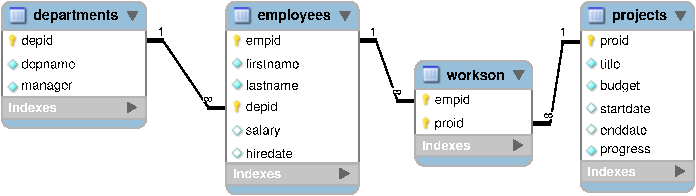
\includegraphics[scale=0.9]{../common/companyREL.pdf}
\end{minipage}
\end{frame}


\begin{frame}[t, fragile, shrink]
\frametitle{Ομαδοποίηση 1:Ν -- βήμα 2}
\begin{minipage}{\wE}
Οι πίνακες {\ra departments} και {\ra employees} έχουν συσχέτιση ένα προς πολλά,
το πεδίο {\ra employees.depid} είναι {\cee ξένο κλειδί}.
\pause
\begin{block}{Σύνδεση πινάκων:}
\[
  departments  \bowtie_{departments.depid  = employees.depid} employees
\]
\vspace*{-1em}
\en
\begin{SQL}
    FROM departments  INNER JOIN employees
         ON departments.depid  = employees.depid
\end{SQL}
\el
\end{block}
\pause
\begin{block}{ή με τη χρήση ψευδωνύμων των πινάκων:}
\[
   \varrho_{d}(departments)  \bowtie_{d.depid = e.depid}  \varrho_{e}(employees)
\]
\vspace*{-1em}
\en
\begin{SQL}
    FROM employees e INNER JOIN departments d
                     ON e.depid = d.depid
\end{SQL}
\el
\end{block}
\end{minipage}
\end{frame}



\begin{frame}[t, fragile, shrink]
\frametitle{Ομαδοποίηση 1:Ν -- βήμα 3}
\begin{minipage}{\wE}
  \begin{block}{Περιορισμός εγγραφών}
Υπάρχει ο περιορισμός για τον μισθό των υπαλλήλων στο ερώτημα.
Επομένως πρέπει να συμπληρωθεί ο όρος \twhere:
\[
   \sigma_{e.salary > 1300}
   (
     \varrho_{d}(departments)  \bowtie_{d.depid = e.depid}  \varrho_{e}(employees)
   )
\]
\pause
\en
\begin{SQL}
    FROM employees e INNER JOIN departments d
         ON e.depid = d.depid
   WHERE e.salary > 1300
\end{SQL}
\el
  \end{block}
\end{minipage}
\end{frame}



\begin{frame}[t, fragile, shrink]
\frametitle{Ομαδοποίηση 1:Ν -- βήμα 4}
\begin{minipage}{\wE}
  \begin{block}{}
Η φράση {\cbb «ανά τμήμα»} δηλώνει ομαδοποίηση, επομένως χρειαζόμαστε τη συμπλήρωση  όρου {\sq \tgroupby}.
Η ομαδοποίηση χρειάζεται για τον υπολογισμό του πλήθους ({\sq COUNT}) {\cbb «ανά τμήμα»}.

\[
  \begin{split} 
   {}_{d.depname} \calg_{count(*)}
   (
     \sigma_{e.salary > 1300}  \\
     (
       \varrho_{d}(departments)  \bowtie_{d.depid = e.depid}  \varrho_{e}(employees)
     )
   )
  \end{split} 
\]
\pause
\en
\begin{SQL}
    FROM employees e INNER JOIN departments d
         ON e.depid = d.depid
   WHERE e.salary > 1300
GROUP BY d.depname
\end{SQL}
\el
  \end{block}
\end{minipage}
\end{frame}



\begin{frame}[t, fragile, shrink]
\frametitle{Ομαδοποίηση 1:Ν -- βήμα 5}
\begin{minipage}{\wE}
\vspace{-1em}
\begin{block}{Προβολή πεδίων}
Από το σύνολο των πεδίων που διατίθενται μετά τη σύζευξη των πινάκων {\ra employees} και {\ra departments}
μας ζητούνται μόνο το όνομα του τμήματος (άρα {\ra departments.depname})
και το πλήθος εργαζομένων ανά τμήμα, δηλαδή  {\ra COUNT(employees.depid)}:
\[
  \begin{split}
   {}_{d.depname} \calg_{count(*) }
   (
     \sigma_{e.salary > 1300}  \\
     (
       \varrho_{d}(departments)  \bowtie_{d.depid = e.depid}  \varrho_{e}(employees)
     )
   )
  \end{split} 
\]
\pause
\en
\begin{SQL}
  SELECT d.depname, COUNT(e.depid)
    FROM employees e INNER JOIN departments d
         ON e.depid = d.depid
   WHERE e.salary > 1300
GROUP BY d.depname
\end{SQL}
\el
  \end{block}
\end{minipage}
\end{frame}


\begin{frame}[t, fragile, shrink]
\frametitle{Ομαδοποίηση 1:Ν -- βήμα 6}
\begin{minipage}{\wE}
  \begin{block}{Επιπλέον επιλογές και παρατηρήσεις}
     \begin{enumerate} \itemsep 6pt
       \item \pause Δεν υπάρχει κάποια απαίτηση για περιορισμό των εγγραφών
             μετά την ομαδοποίηση, δεν χρειάζεται ο όρος {\sq HAVING}.
       \item \pause  Δεν υπάρχει απαίτηση για ταξινόμηση των εγγραφών του αποτελέσματος,
             δεν χρειάζεται ο όρος {\sq ORDER BY}.
       \item \pause  Το ερώτημα είναι πλήρες λοιπόν.      
    \end{enumerate}
  \end{block}
\end{minipage}
\end{frame}



\begin{frame}[t, fragile, shrink]
\frametitle{Ομαδοποίηση 1:Ν -- Τελική διατύπωση}
\begin{minipage}{\wE}
  \vspace*{-0.6cm}
  \begin{exampleblock}{\small Να βρεθεί το πλήθος των εργαζομένων με μισθό μεγαλύτερο των 1300 \euro\ ανά όνομα τμήματος}
  \pause
  \en
\begin{SQL}
  SELECT d.depname, COUNT(e.depid)
    FROM employees e INNER JOIN departments d
         ON e.depid = d.depid
   WHERE e.salary > 1300
GROUP BY d.depname
 
 depname                          COUNT(*)
------------------------------------------
&mgr{ Γραμματείας              }               1
&mgr{ Διοίκησης/Επίβλεψης      }               3
&mgr{ Εξωτερικών συνεργατών    }               1
&mgr{ Επιστημόνων/Μηχανικών    }               3
&mgr{ Μάνατζμεντ/Πωλήσεων      }               5
&mgr{ Οικονομoλόγων/Λογιστών   }               3
\end{SQL}
\el
\end{exampleblock}
\end{minipage}
\end{frame}

